\documentclass{book}

\usepackage{fullpage}

%\usepackage{wrapfig}
%\usepackage{float}
%  \floatstyle{ruled}
%  \newfloat{callout}{thp}{lop}
%  \floatname{callout}{Things To Remember}

\usepackage{color}
\definecolor{Light}{gray}{.95}

\usepackage{amsthm}
{
  \theoremstyle{definition}
  \newtheorem{example}{Example}
}

\usepackage{graphicx}

\newlength{\calloutparindent}
\setlength{\calloutparindent}{\parindent}
%%
%% begin: the callout command
\newcommand{\callout}[3]{\label{#1}\vspace{3mm}
\begin{center}
\fcolorbox{black}{Light}{\begin{minipage}{0.85\textwidth}
    \textbf{\large Things To Remember~\ref{#1} --- #2}
    \hrule
    \vspace{2mm}
\setlength{\parindent}{\calloutparindent}
#3
  \end{minipage}}
\end{center}
\vspace{3mm}
}
\newcommand{\thingstoremember}[1]{Things To Remember~\ref{#1}}
%% end: the callout command
%%

% two chapters will precede the one here now
\setcounter{chapter}{3}

\begin{document}

\chapter{Delegation}

An important design decision when modeling data is how many Java classes to use to represent an entity. At one extreme, an entity is stuffed into a single class, resulting in a coarse-grained design. At the other extreme, a main entity class delegates functionality to other classes, resulting in a fine-grained design.  Delegation is a very popular pattern because of the flexibility it provides. 

Programmers rarely think about memory costs when deciding how to model entities. Yet, the choices made at this design stage impact memory costs significantly. Coarse-grained designs may result in many objects with unused fields. While delegation is sometimes a way to avoid this problem, overly fine-grained data models can result in poor memory health from excessive object header overhead. This chapter explains how to evaluate object granularity design choices from a memory perspective. It begins with the costs of basic objects, and works up to examples from real applications.
  
\section{The Cost of Objects}


There is no Java library method that returns the size of an object. This is by design. A Java programmer is not supposed to know either the size of an object or how it is layed out in memory. But if you know the costs of the built in primitives and types, it is not hard to compute a reasonable estimate.
\footnote{You can obtain the exact size of an object using the Sun HPROF agent.}  

Java specifies the sizes needed to store primitive types:
\begin{table}
  \centering
 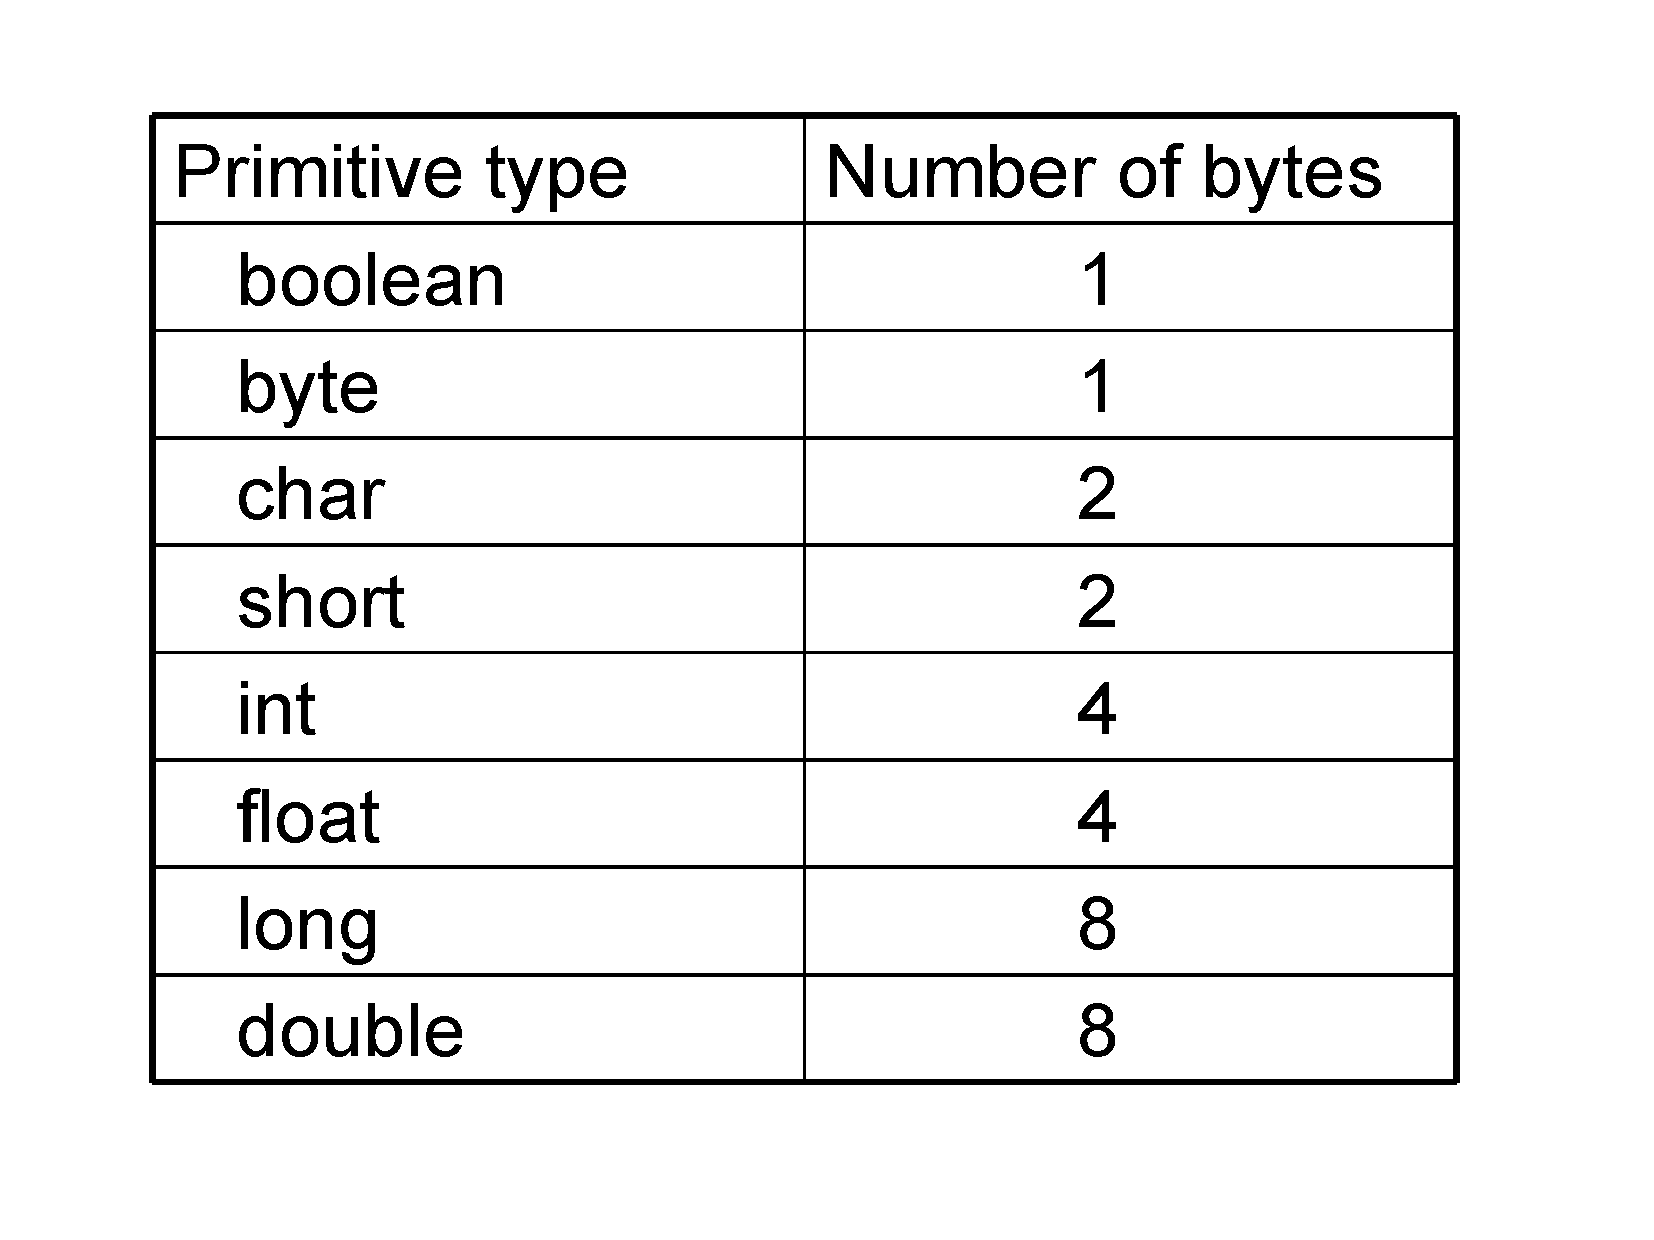
\includegraphics[width=.40\textwidth]{Figures/chapter4/primitive-byte-sizes.pdf}
 % 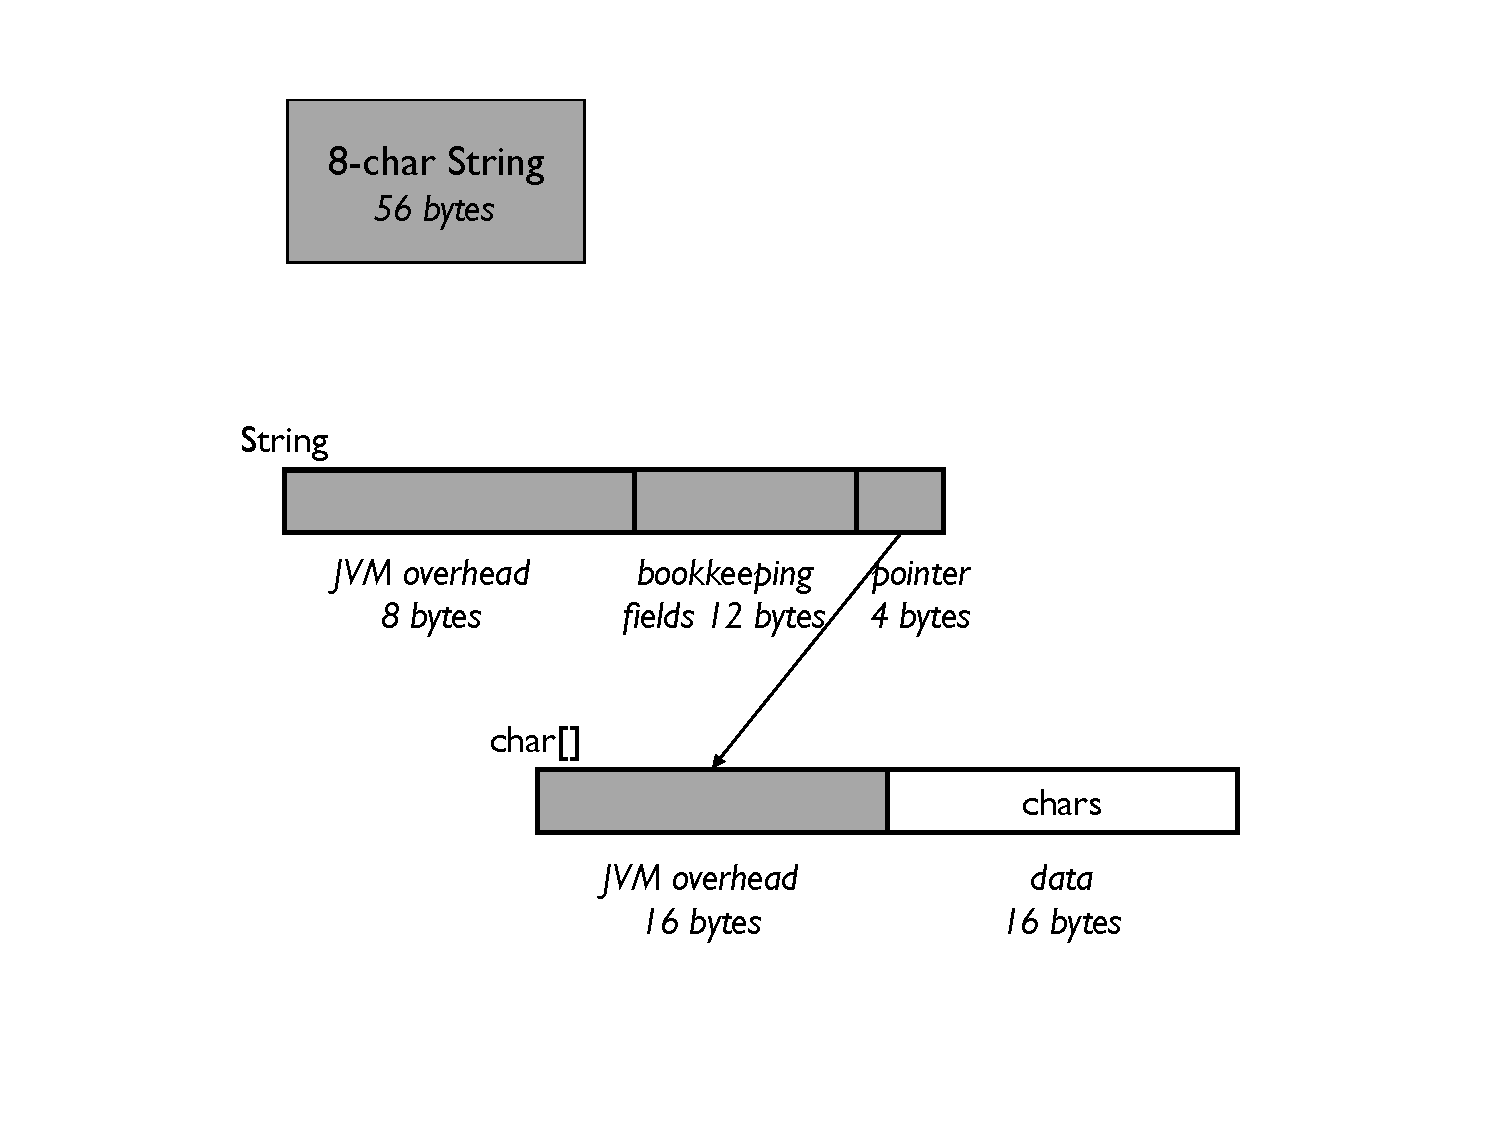
\includegraphics{eight-char-string}
  \caption{The sizes of Java primitive types}
  \label{tab:primitive-sizes}
\end{table}

Objects are much bigger. Both the JVM and the hardware impose costs, which are substantial for small objects. These costs can differ, depending on the JVM and on the hardware. For now, all sizes are for 32-bit architectures. Each object has a header that stores information that the JVM and garbage collector needs, such as the class, an active monitor and an identity hashcode. 

The underlying hardware can impose alignment costs. The hardware may require 2-byte, 4-byte, or 8-byte alignment, depending on the type of the data. For example, integers are usually aligned on a 4-byte boundary, and some hardware might require a double to be aligned on an 8-byte boundary. A JVM may impose an alignment requirement above and beyond the hardware, if there is some performance benefits for storage allocation and garbage collection.  

The Sun 6u1.4 JVM allocates 8 bytes per object header, and the IBM J9 JVM allocates 12 bytes per header. Both the 6u1.4 and J9 JVMs allocate objects on 8-byte boundaries. That means that the size of any object is a multiple of 8, and the smallest object is 16 bytes, assuming it holds at least one piece of data. The header takes at least 8 bytes, and with at least one additional byte for data, the alignment requirement forces an object to be at least 16 bytes. The table~\ref{tab:boxed-scalar-sizes} gives the sizes for boxed scalars.

\begin{table}
  \centering
 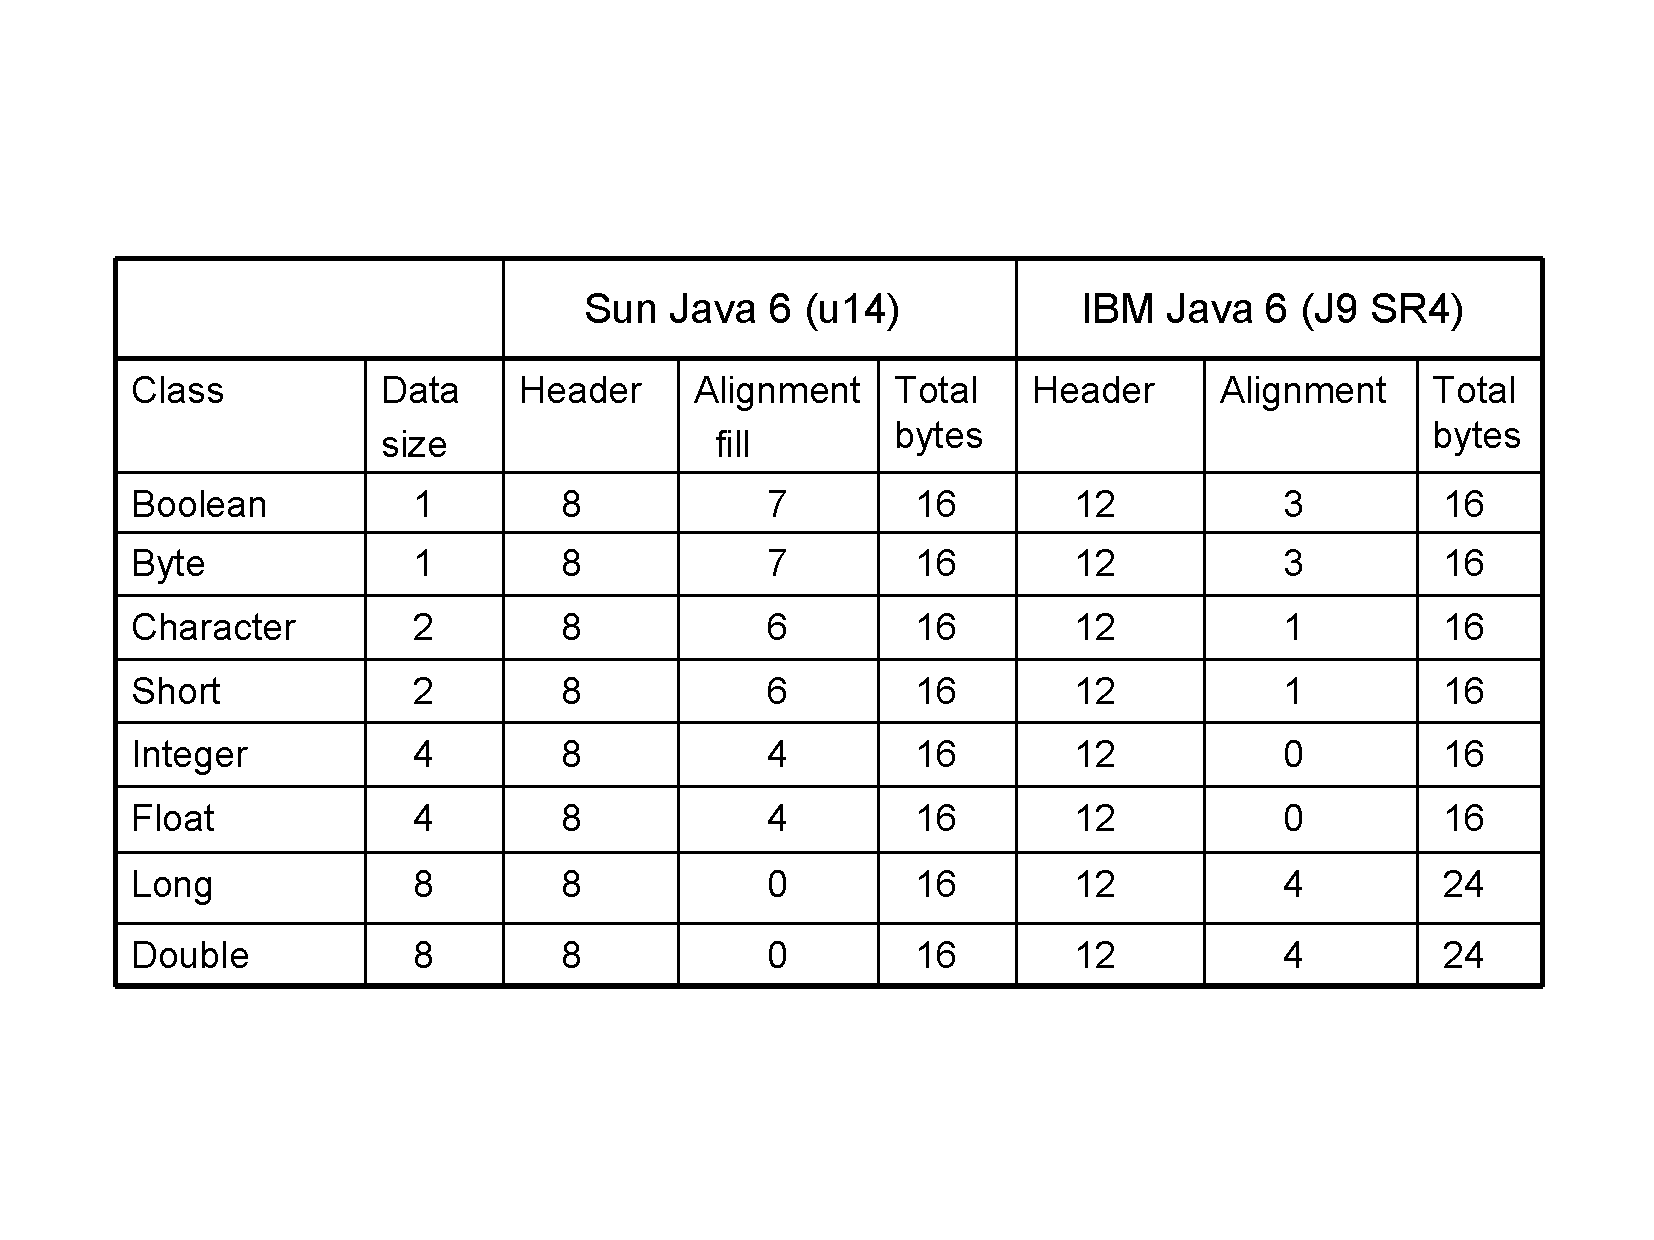
\includegraphics[width=.40\textwidth]{Figures/chapter4/boxed-scalar-sizes.pdf}
 % 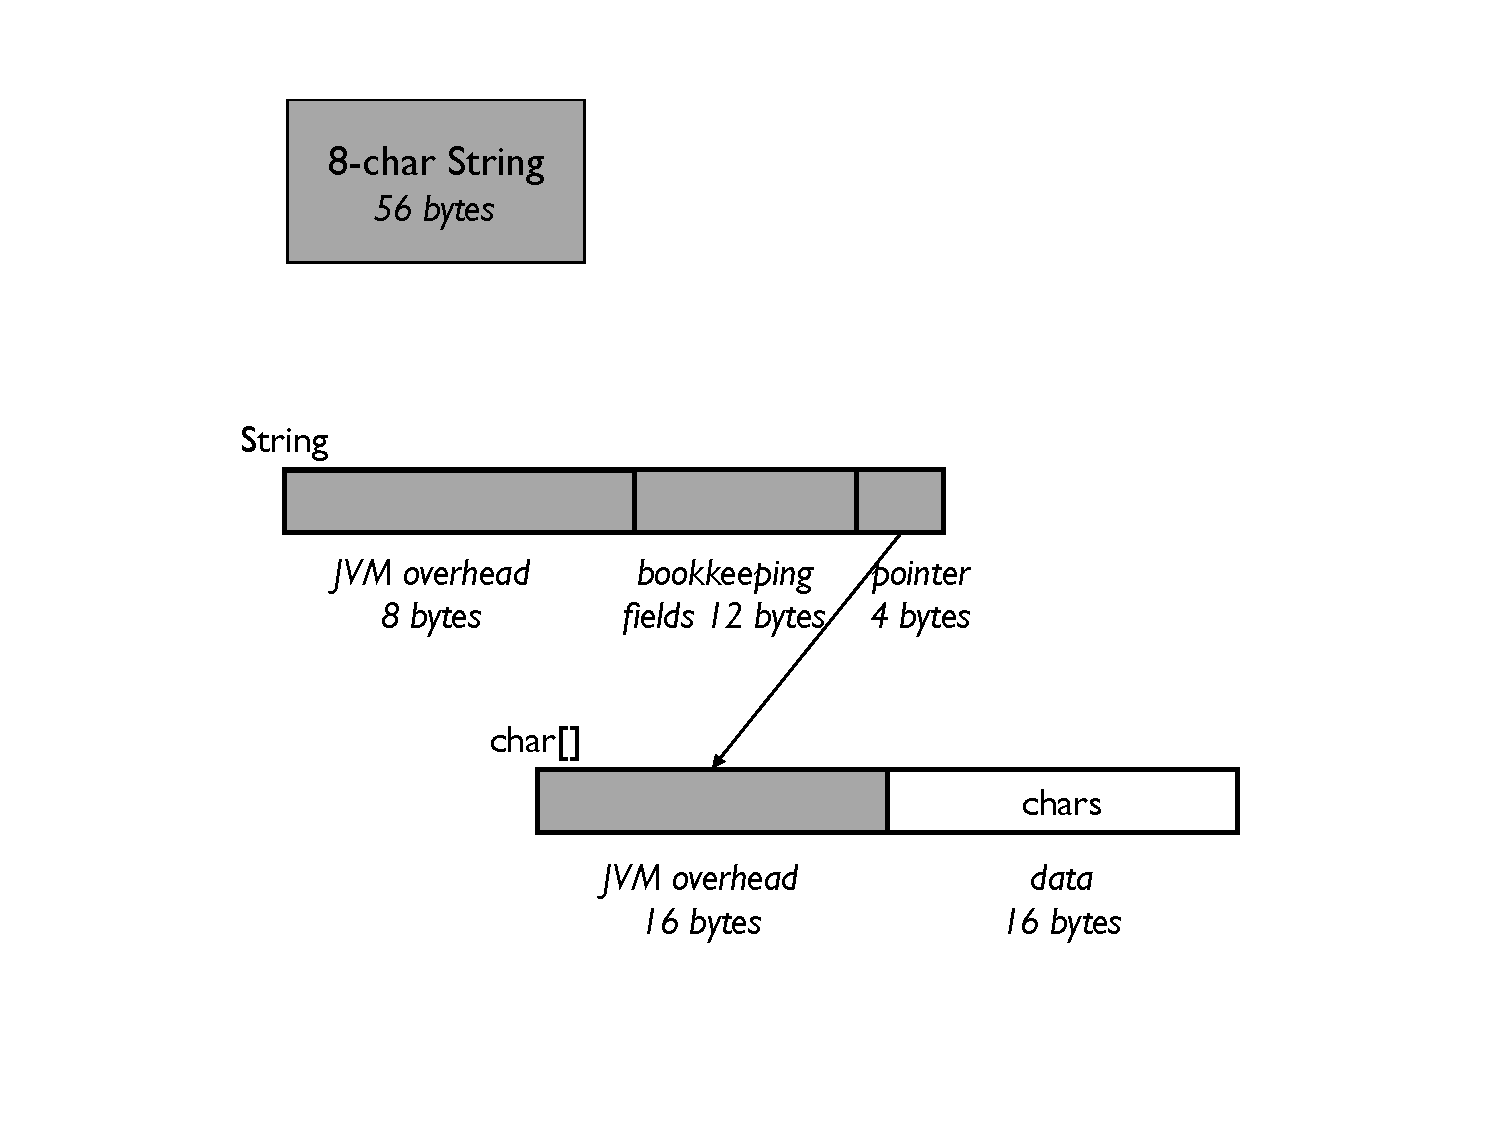
\includegraphics{eight-char-string}
  \caption{The sizes of boxed scalar objects.}
  \label{tab:boxed-scalar-sizes}
\end{table} 

There is a simple rule that holds here. The size of the object is obtained by adding together the size of the header and the data, and then rounding it up to the nearest multiple of 8. The generalization of this rule gives you a good way to estimate the size of any object. Often, this estimate turns out to be the real object size, but not always. The JVM has freedom in the way it lays out an object. 
 
\callout{callout:object-size-estimation-rule}{Minimum Size Estimation Rule}{
    Let $Header$ be the size of an object header, and $Alignment$ be the object alignment required by a JVM. That is, every object must be allocated at an address which is a multiple of $Alignment$. You can estimate the minimum size of an object by 1) summing up the sizes of all of the data stored in the object, including data from superclasses, 2) adding this sum to $Header$, and 3) rounding the result up to the next multiple of $Alignment$. 
}

The rule works the same way for array objects, except that there is always an additional 4 bytes in the header to store the number of elements. 

\begin{example}[Employee class and subclass.]
Consider a \texttt{EmployeeStatus} class defined as follows:

\ttfamily
\begin{verbatim} 

			class EmployeeStatus {
			  int hoursPerWeek;
			  boolean exempt;
				double salary;
				char jobCode;
				int yearsOfService;
			}
\end{verbatim}
\normalfont
Applying the size estimation rule, and assuming both $Header$ and $Alignment$ are 8 bytes JVM, the minimum size of an \texttt{EmployeeStatus} object is 32 bytes. You first add (4+1+8+2+4)+8 which is 27, and then round to the next multiple of 8, resulting in 32 bytes.  If the header is 12 bytes, then the estimated size is also 32 bytes, since (4+1+8+2+4)+12 is 31, which still rounds up to 32.

How accurate are these estimates for the reference JVMs? For Java 6u14, this estimation technique works very well. This is because 6u14 does a good job in packing fields. 

			class EmployeeOnLeave extends EmployeeStatus {
				int numLeaveMonths;
			}
			
\end{example}

In fact, according to HPROF, the size of an \texttt{EmployeeStatus} object is precisely 32 bytes.


So just lets talk a little about what this means for 64-bit JVMs. People are busting out of this 32-bit address space now, and they are saying let's go to 64-bit, and that will solve everything. Unfortunately, when you go to 64-bit, things blow up pretty quickly. , the object headers are double, pretty sure that's the same thing in sun. arrays are not quite double. 24 bytes. The other thing is that all the pointers instead of being 4 bytes, are now 8 bytes; and finally, there's still that same alignment cost in J9. In SUN you will have a higher alignment cost, since in SUN now it's aligned to 8-byte boundary, where it was aligned to 4-byte boundary before.  The studies I've read, both outside and inside IBM, are showing that going to a 64-bit JVM will increase your memory usage by 40-50\%, and I've heard arguments that say that yur application will run faster, because of the native architecture and all that,  but in some cases there is evidence that it may run slower, because of the worse cache locality. It's another example where it's super important to measure, and not make assumptions that this will fix my speed problem, or it will fix my memory problem. There are a lot of surprises in this area. So J9, and some of the other JVMs, I don't think SUN has this yet, I coud be wrong, I know JRocket has it , they have a mode have called compress addressing, where they can squeeze a few extra bits out of the 32-bit addresses, and in J9 6SR2 is going to allow addressing of up to 28 gig with a 32 bit address still, so without all of these additional footprint problems, if you use this compressing flag. From what I've read, it's only a few percentage degradation in performance, it's pretty minor, so it can certainly help people in this transition area.




\callout{callout:memory-bloat-factor}{The Memory Bloat Factor}{
    An important metric for evaluating the health of a data model
    design is the fraction of overhead in the objects of that data
    model. The \emph{memory bloat factor}, or simply \emph{bloat
      factor}, is the ratio of overhead to total size. 
}
% TODO: add alignment
%\begin{figure}
%  \centering
%  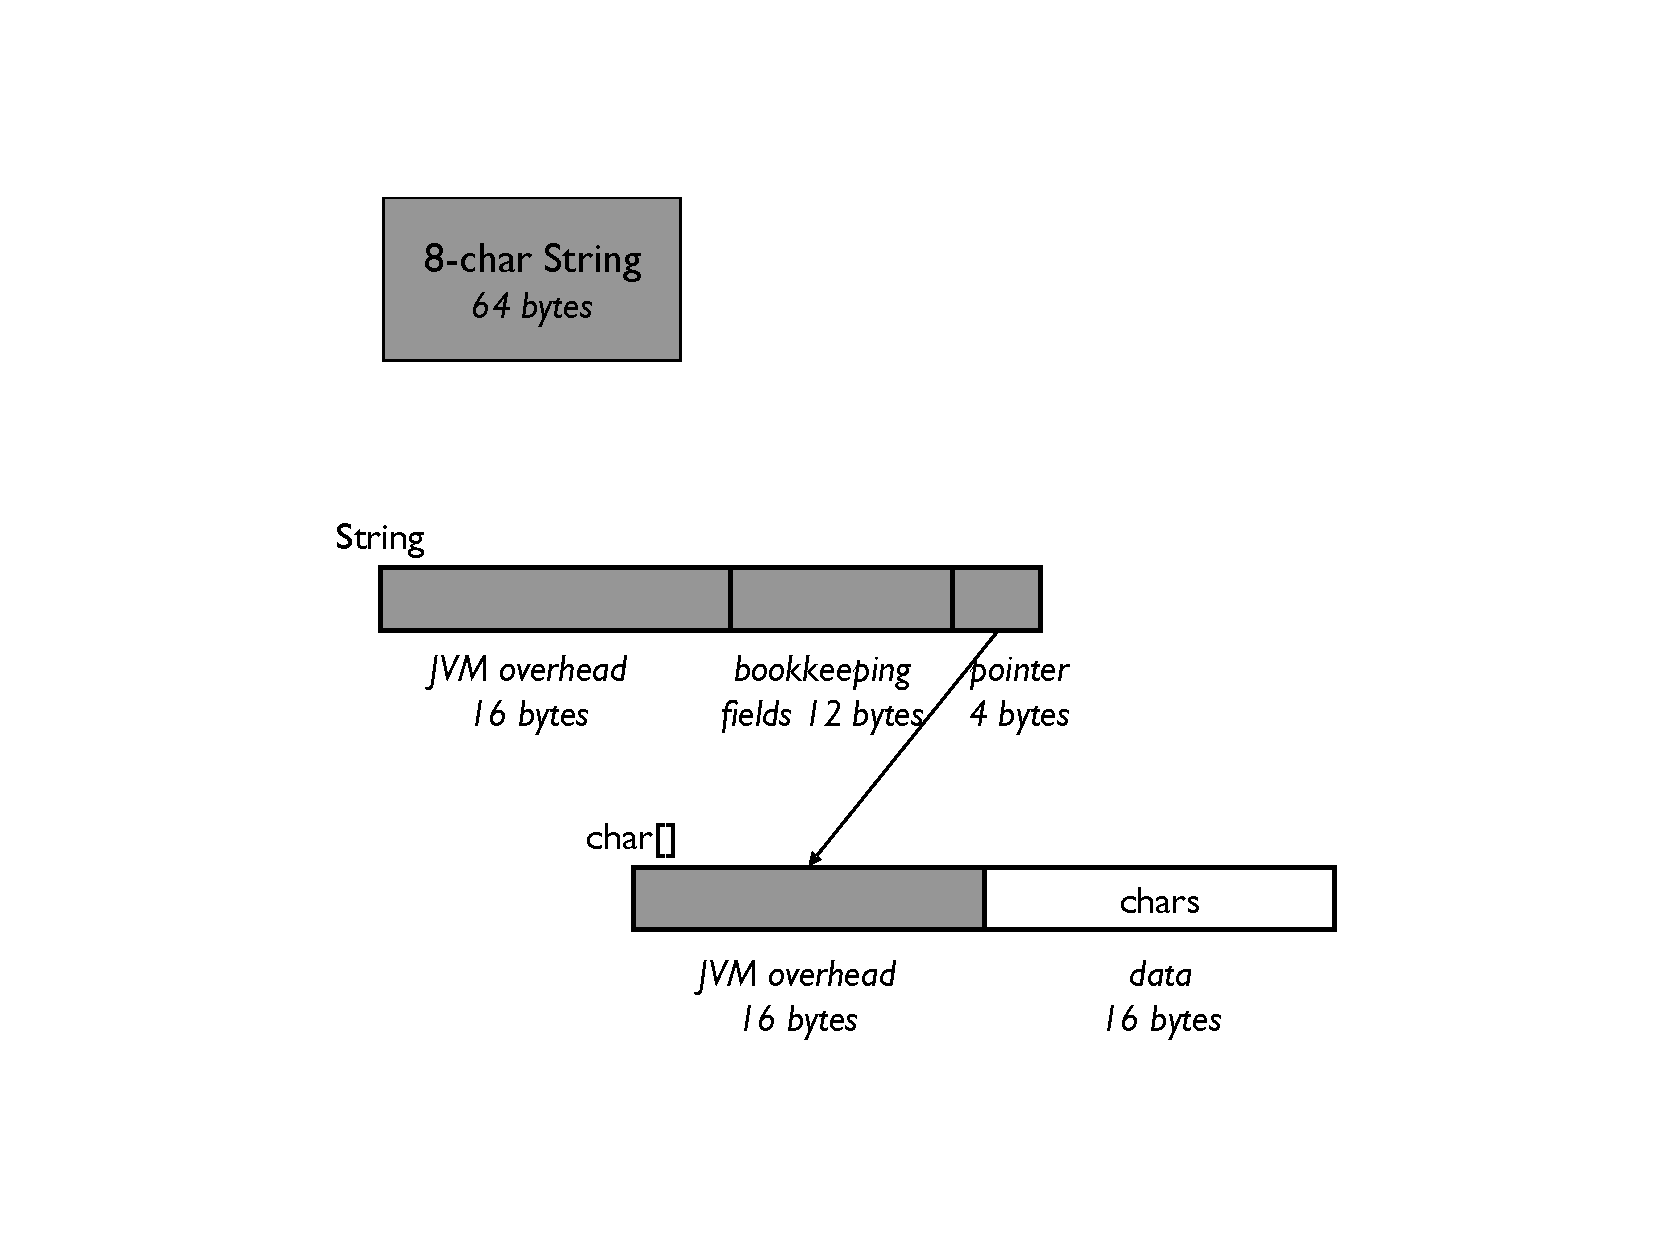
\includegraphics[width=.70\textwidth]{Figures/chapter3/eight-char-string.pdf}
  %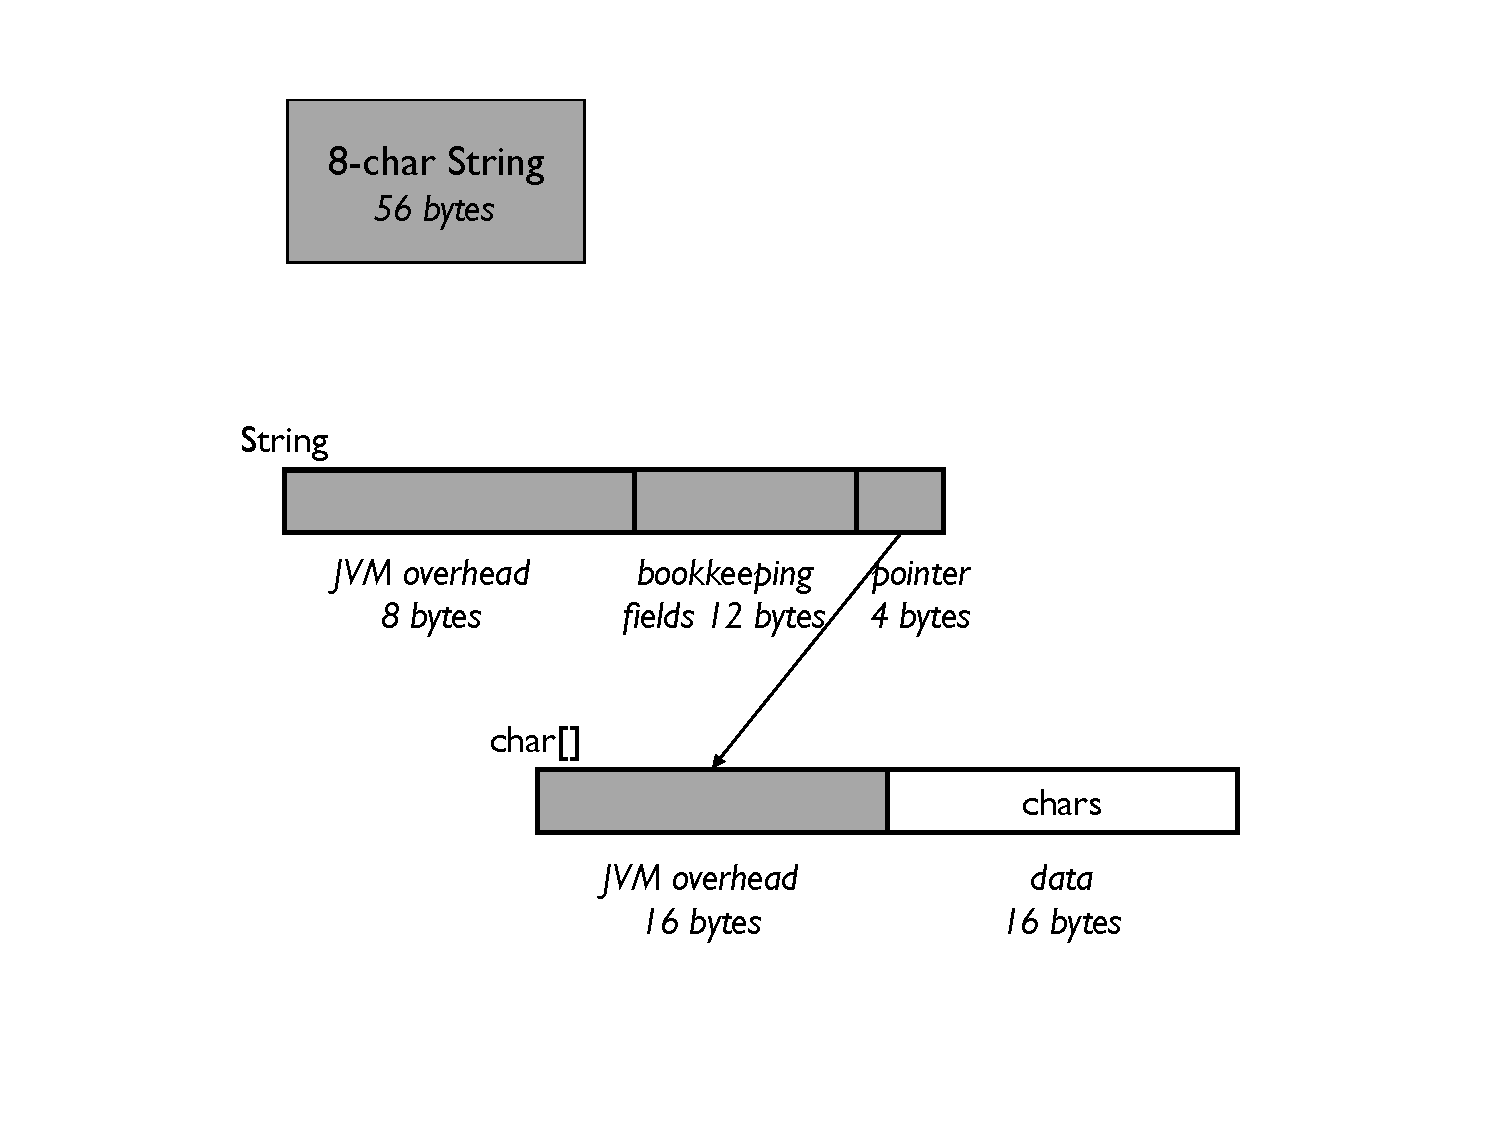
\includegraphics{eight-char-string}
%  \caption{An eight character string in Java 6.}
 % \label{fig:eight-char-string}
%\end{figure}

\section{The Cost of Delegation}


\section{Fine-Grained Data Models}
\label{fine-grained-data-models} 

\section{Large Base Classes}

\section{Summary}


\end{document}
